\chapter{Revisão de Literatura}
  
  Este capítulo apresenta a revisão de literatura realizada sobre os assuntos pertinentes ao trabalho, abordando
  tópicos como metodologias ágeis e estimativa e processos de medição.
  
\section{Planejamento e estimativas em metodologias ágeis}

  As metodologias ágeis se baseiam nos valores ágeis publicados no Manifesto Ágil
  (BECK, 2001 \textit{apud} \citeonline{cohn06}), que são:

  \begin{itemize}
   \item Indivíduos e interações entre eles mais que processos e ferramentas;
   \item Software em funcionamento mais que documentação abrangente;
   \item Colaboração com o cliente mais que negociação de contratos;
   \item Responder a mudanças mais que seguir um plano.
  \end{itemize}

 Seguir uma metodologia ágil em um projeto, também implica em uma abordagem ágil nas estimativas e planejamento, seguindo
 os valores supracitados \cite{cohn06}. Conceitos importantes são necessários para entender o planejamento e estimativas
 num projeto ágil, como: iteração e \textit{sprints}, \textit{story points}, \textit{velocity}, entre outros.
 Esses conceitos serão devidamente aprofundados nas próximas seções.

  \subsection{Tempo de trabalho: \textit{Sprints}}

    Times ágeis trabalham em iterações, que são um período de tempo fixo (\textit{time-boxed}) curto, de não mais que
    um mês de duração \cite{cohn06} \cite{scrum13}. O \textit{Scrum}, um \textit{framework} estrutural ágil,
    traz o conceito de \textit{Sprint} para o processo de desenvolvimento, que nada mais é que um \textit{container}
    temporal fixo para outros eventos do \textit{Scrum} \cite{scrum13}. Numa \textit{Sprint} é produzido um incremento
    do \textit{software}, com base no que foi estabelecido como escopo daquela \textit{Sprint}. Como uma \textit{Sprint} possui
    a duração fixa, mesmo que uma funcionalidade não tenha sido completada nesta \textit{Sprint}, a mesma é encerrada no prazo
    que foi determinado \cite{cohn06}.

    De acordo com \citeonline{scrum13}, a
    \textit{sprint} é composta pela reunião de planejamento da \textit{sprint}, reuniões diárias, trabalho de desenvolvimento,
    revisão da \textit{sprint} e retrospectiva da \textit{sprint}. Os esforços de estimativas se concentram na reunião de
    planejamento da \textit{sprint}, onde são estimadas as histórias de usuários. No começo de cada \textit{sprint}, o time
    incorpora todo o conhecimento obtido com a \textit{sprint} passada para adaptar e ajustar o planejamento da próxima
    \textit{sprint} \cite{cohn06}.

  \subsection{Estimativas com \textit{Story Points}}

    Em um projeto ágil
    que utiliza histórias de usuário, pode-se estimar o tamanho de uma história em \textit{story points}.
    \textit{Story points} representam o tamanho geral de uma história, envolvendo o esforço necessário, a complexidade e os
    riscos inerentes para desenvolver a história \cite{cohn06}. O número atribuído à história como seu tamanho não é relevante,
    o que importa é o valor relativo entre as histórias, que é obtido por comparação entre elas \cite{cohn06}.

      \subsubsection{\textit{Velocity}}

	Numa abordagem ágil, a estimativa do tamanho é separada da estimativa da duração \cite{cohn06}.
	Com o tamanho estimado, é preciso de outro conceito para se calcular a duração, o \textit{velocity}.
	O \textit{velocity} mede a taxa de progresso do time, dizendo quantos pontos o time é capaz de desenvolver
	numa \textit{sprint}, podendo ser calculado como a soma dos pontos concluídos durante a iteração \cite{cohn06}.
	A melhor forma de se estabelecer o \textit{velocity} para um time é executando uma ou duas iterações e estimar o
	\textit{velocity} a partir do \textit{velocity} observado \cite{cohn06}.

      \subsubsection{Estimando a duração}

	Com o tamanho do \textit{software} e o \textit{velocity} do time de desenvolvimento conhecido, fica fácil estimar
	um prazo para o projeto, dividindo o tamanho pelo \textit{velocity}, obtendo assim a quantidade de \textit{sprints}
	necessárias, e multiplicando pelo tamanho da \textit{sprint} \cite{cohn06}.

	Utilizando uma abordagem por \textit{story points} em um projeto, separa-se completamente a estimativa do esforço
	necessário da estimativa da duração do projeto, permitindo que ambos sejam estimados independentemente. A estimativa de
	duração do projeto passa a ser derivada da estimativa de esforço \cite{cohn06}.

      \subsubsection{Escala das estimativas}
      \label{estimation_scales}

	  Utilizar uma única ordem de magnitude gera estimativas melhores (Miranda 2001; Saaty 1996 \textit{apud} \cite{cohn06}).
	  De acordo com \citeonline{cohn06}, uma escala de estimativa bastante utilizada e que se mostra bastante eficaz é a
	  sequência \textit{Fibonnaci}, que consiste em pontuar as histórias utilizando algum número da
	  sequência 1, 2, 3, 5, 8, 13, [...]. É importante estabelecer um valor máximo para a sequência para manter o intervalo
	  conhecido e não demasiado grande.

      \subsubsection{\textit{Planning Poker}}

	O \textit{Planning Poker} é uma técnica utilizada para estimativas ágeis que envolve as três técnicas de estimativa
	mais comuns (opinião do especialista, analogia e desagregação), gerando estimativas rápidas e confiáveis \cite{cohn06}.

	Todos os desenvolvedores participam do \textit{Planning Poker}, que se inicia com a entrega das cartas que contém os
	valores válidos para as histórias na escala definida (vide a sub-seção \ref{estimation_scales}).
	Uma história é selecionada e é lida sua descrição pelo moderador
	do jogo (usualmente o \textit{Product Owner}, que não participa das estimativas) para que então os jogadores possam
	avaliar a história e pontuá-la. Se houver divergências entre as pontuações, é iniciado um debate para que seja definida
	a pontuação final da história. Uma nova rodada é jogada para a mesma história caso os participantes não
	entrem em um consenso \cite{grenning02}.

	O objetivo é fazer com o que os participantes convirjam para uma estimativa que será utilizada como pontuação da
	história, lembrando que a proposta do \textit{Planning Poker} não é gerar uma estimativa acurada que perdure por
	todo o ciclo de desenvolvimento, pois para atingir tal estimativa seria gasto um esforço
	desnecessário \cite{cohn06} \cite{grenning02}.

	\citeonline{cohn06} diz que existe uma acurácia máxima para uma estimativa
	em relação ao esforço necessário para realizá-la, como ilustra a Figura \ref{fig:effort_accuracy}.
	Portanto, não é preciso um debate demorado e detalhado durante o \textit{Planning Poker} para se definir
	o tamanho das histórias, objetivando sempre ficar do lado esquerdo da curva apresentada na Figura \ref{fig:effort_accuracy}.

	\begin{figure}[!htb]
	  \centering
	  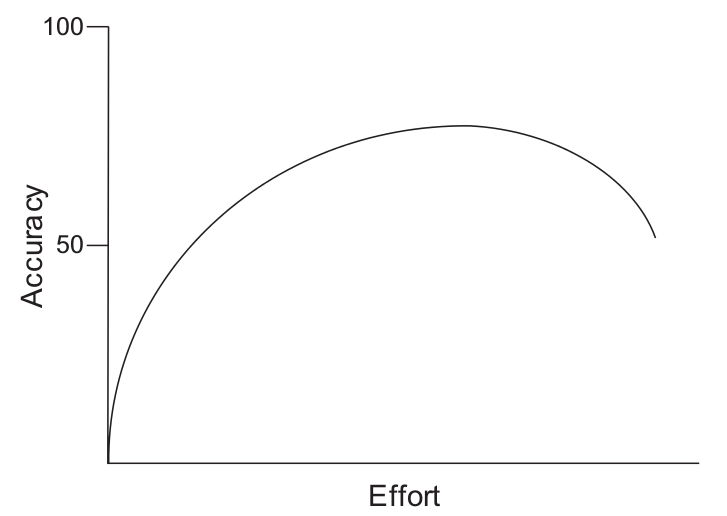
\includegraphics[scale=0.4]{figuras/effort_accuracy}
	  \caption[Relação entre a acurácia e o esforço realizado para a estimativa.]
		  {Relação entre a acurácia e o esforço realizado para a estimativa. Fonte: \cite{cohn06}}
	  \label{fig:effort_accuracy}
	\end{figure}

  \subsection{\textit{Burndown}}

    Objetivando conhecer a velocidade com a qual a equipe realiza seu trabalho, elabora-se um gráfico \textit{burndown} o qual é responsável por mostrar a quantidade de trabalho restante no início de cada iteração. Além disso, essa ferramenta se torna um poderoso indicador visual da rapidez com que uma equipe está se movendo em direção a sua meta \cite{cohn06}. O \textit{burndown} pode ser calculado por \textit{sprint}, por \textit{release}, por um projeto como um todo. No âmbito deste trabalho foi trabalhada a ideia de realização de \textit{burndown} por \textit{sprint}.

    Em um gráfico \textit{burndown} por \textit{sprint} apresenta-se no eixo vertival o número de pontos de história restantes na sprint e no eixo horizontal os dias ao longo da \textit{sprint} \cite{cohn06}.

\section{Processo de medição}
  
  "Medição é o processo pelo qual números ou símbolos são designados a atributos de entidades do mundo real para descrevê-los de 
  acordo com regras claramente definidas" \cite{fenton97}. Para \citeonline{solingen99}, medição de \textit{software} é o processo
  contínuo de definir, coletar e analisar dados obtidos no processo de desenvolvimento de \textit{software} para entender e controlar
  o processo e seus produtos, bem como fornecer informações para melhorá-los.

  Para atingir o objetivo do trabalho, será necessário a utilização de um processo de medição para obter informações a respeito
  dos fatores de atraso identificados. Para a definição do processo de medição temos diversas abordagens, onde algumas serão
  descritas nesta seção.
  
  \subsection{Norma ISO/IEC 15939:2007}
  
      A norma ISO/IEC 15939 define atividades e tarefas necessárias para implementar um processo de medição, adaptado do 
      ciclo de melhoria \textit{Plan-Do-Check-Act} (PDCA) \cite{iso15939}. Uma característica importante desta norma é que 
      ela traz o conceito de compromisso com o processo de medição, pois é necessário que a organização esteja comprometida
      com o processo de medição para que a organizaçõa colabore com as medições e que o processo não seja um fracasso.
      
      Segundo a ISO/IEC 15939, o processo de medição consiste em quatro atividades sequenciadas em um ciclo iterativo,
      conforme ilustra a Figura \ref{iso15939_model}. São elas \cite{iso15939}:
      
      \begin{itemize}
	
	\item \textbf{Estabelecer e manter o compromisso com o processo de medição} - Compreende as tarefas para definir os requisitos
	      de medição (o compromisso com a medição é um deles) e alocar recursos;
	      
	\item \textbf{Planejar o processo de medição} - Compreende as tarefas de caracterização da organização, identificação das 
	      necessidades de informação, selecão das métricas e definição dos aspectos necessários à coleta e avaliação de dados e 
	      a comunicação dos resultados;
	      
	\item \textbf{Executar o processo de medição} - Compreende as tarefas de integração dos procedimentos de geração e coleção
	      de dados e de análise e comunicação dos dados, coleta de dados, análise dos dados e elaboração dos produtos de
	      informação e comunicação dos resultados aos interessados;
	
	\item \textbf{Avaliar o processo de medição} - Compreende as tarefas avaliação dos produtos de informação gerados e do
	      próprio processo de medição e identificação de melhorias potenciais.
	
      \end{itemize}

      \begin{figure}[!htb]
	\centering
	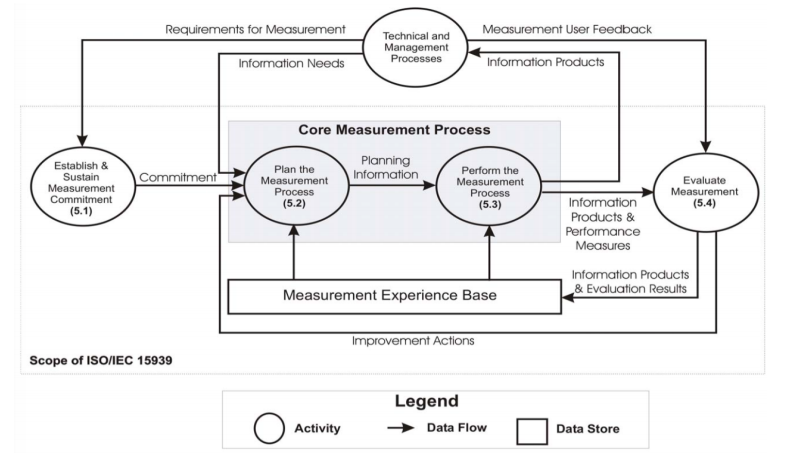
\includegraphics[scale=0.55]{figuras/iso15939}
	\caption[Modelo do processo proposto pela ISO/IEC 15939:2007.]
		{Modelo do processo proposto pela ISO/IEC 15939:2007. Fonte: \cite{iso15939}}
	\label{iso15939_model}
      \end{figure}
      
      Pela Figura \ref{iso15939_model} é possível ver que o processo proposta por esta norma é dirigido por
      necessidades de informação da organização \cite{iso15939}.

  \subsection{Método \textit{Goal-Question-Metric} (GQM)}
  
    O GQM representa uma abordagem sistemática para a adequação e integração de objetivos para modelos do processo de software,
    que defende que a medição deve ser orientada a objetivos (Basili et al, 1994 \textit{apud} \cite{solingen99}). 
    \citeonline{solingen99} afirma que "o resultado obtido com a aplicação do GQM é a especificação de uma programa
    de medição direcionado para um conjunto particular de problemas e um conjunto de regras para a interpretação dos dados da medição".
    
    O modelo do GQM propõe uma abordagem \textit{top-down} para a definição das métricas e uma \textit{bottom-up} para a interpretação
    das métricas, como ilustra a Figura \ref{gqm_model}.
    
    \begin{figure}[!htb]
      \centering
      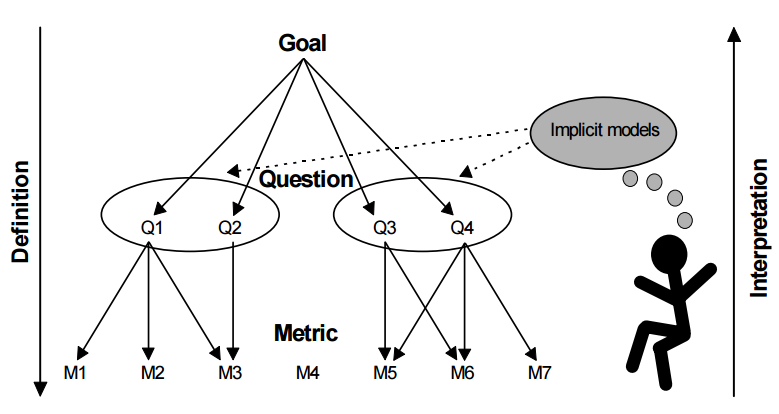
\includegraphics[scale=0.5]{figuras/gqm_model}
      \caption[Modelo do GQM.]
	      {Modelo do GQM. Fonte: Basili et al, 1994 \textit{apud} \cite{solingen99}}
      \label{gqm_model}
    \end{figure}
    
    Assim como ilustra a Figura \ref{gqm_model}, para o processo de definição de métricas, primeiramente são estabelecidos objetivos
    de medição, que devem estar alinhados com os objetivos de negócio da organização,
    que então são refinados em questões que atendam a estes objetivos. Cada questão é refinada em métricas que são
    capazes de prover informações que respondam à questão. Já o processo de interpretação é feito a partir das métricas, que respondem
    às questões que as derivaram, cuja questões atendem ao seu objetivo inicial \cite{solingen99}.
    
    O método GQM contém quatro fases, como ilustra a Figura \ref{gqm_phases}, segundo \citeonline{solingen99}:
    
    \begin{itemize}
     
     \item \textbf{Fase de Planejamento}, onde o projeto para aplicação da medição é selecionado, caracterizado e planejado.
     
     \item \textbf{Fase de Definição}, onde o programa de medição é definido e documentado.
     
     \item \textbf{Fase de coleta de dados}, onde os dados necessários são coletados.
     
     \item \textbf{Fase de interpretação}, onde os dados coletados são processados e ocorre o processo de interpretação supracitado.
     
    \end{itemize}
  
    \begin{figure}[!htb]
      \centering
      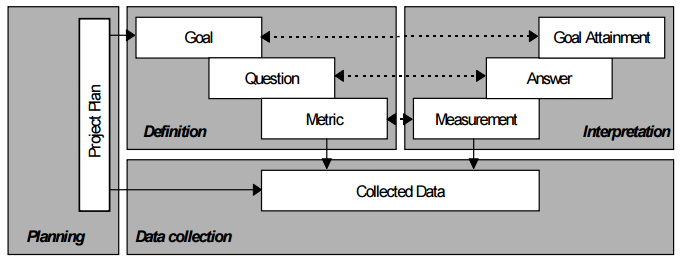
\includegraphics[scale=0.5]{figuras/gqm_phases}
      \caption[Fases do GQM.]
	      {Fases do GQM. Fonte: \cite{solingen99}}
      \label{gqm_phases}
    \end{figure}